\newgeometry{top=2cm, bottom=2cm, left=3cm, right=3cm} %when used with the geometry package, allows you to adjust page margin parameters for each specific page or for a specific section of your document
\setlength{\columnsep}{32pt}
\begin{multicols}{2}
\noindent
уравнений: сначала решается урав- нение (4), корнями которого явля- ются суммы $\epsilon_1+\epsilon_4$ и $\epsilon_2 +\epsilon_3$ симмет- ричных (см. рис. б!) корней уравнения (3), а затем из уравнений (5) находятся и сами корни уравнения(3).\par
Именно таким путем Гауссу удалось осуществить построение правильного 17-угольника: здесь тоже выделяются группы корней, суммы которых находятся последовательно из квадратных уравнений. Но как искать эти <<хорошие>> группы?  Гаусс находит удивительный путь ответить на этот вопрос...\par
\begin{center}
    \textbf{Построение правильного\\
        17-угольника}
\end{center}
\begin{adjustwidth}{1cm}{0cm}
    \scriptsize\textbf{\qquad30 марта 1796 года наступает для него (Гаусса) день творческого крещения... Гаусс уже занимался с некоторого времени группировкой корней из единицы на основании своей теории <<первообразных>> корней. И вот однажды утром, проснувшись, он внезапно ясно и отчетливо осознал, что из его теории вытекает построение семнадцатнугольника... Это событие явилось поворотным пунктом жизни Гаусса. Он принимает решение посвятить себя не филологии, а исключительно математике.}
\end{adjustwidth}
\begin{flushright}    
    \scriptsize\textit{Ф. Клейн}\par
\end{flushright}

    Чтобы выявить найденные Гауссом скрытие <<симметрии>> в множестве корней 17-й степени из единицы и, пользуясь ими, разбить корни на нужные группы, введем новую нумерацию корней. Будем возводить 3 и последовательные степени 0, 1, 2, ,,, и каждый раз брать остаток от деления полученного числа на 17. Избавим читателя от проведения этих выкладок и в таблице приведем окончательные результаты. В первой строке стоят показатели k, а под ними остатки от деления $3\sp{k}$ на 17.\\
    Обратите внимание, что в нижней строке содержатся все числа от 1 до
    \columnbreak
    \begin{figure}[H]
        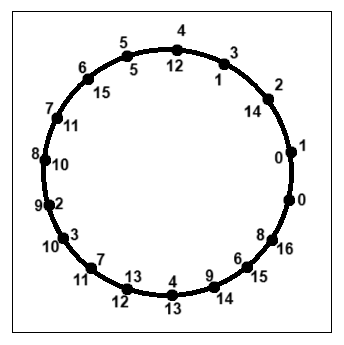
\includegraphics[width=\columnwidth]{Untitled2.png}
    \end{figure}
    \noindent\scriptsize\textbf{Рис. 7. Старые номера корней даны черным цветом, новые - красным}\\[2em]
    \normalsize
    1б; затем $3\sp{16}$ дает остаток 1 и далее остатки периодически повторяются (докажите!)\par
    
    Закономерность, \qquad подмеченная Гауссом, является частным случаем следующей теоремы: д л я в с я к о г о \quad п р о с т о г о \qquad \textit{p} \quad с у щ е с т в у е т \quad т а к о е \quad ч и с л о \quad \textit{l}, \quad н а з ы в а е м о е \quad п е р в о о б р а з н ы м \quad к о р н е м, \quad ч т о \quad с р е д и \quad о с т а т к о в \quad о т \quad д е л е н и я \quad $l\sp{k}$ \quad на p \quad в с т р е ч а ю т с я \quad в с е \quad ч и с л а \quad 1, \quad 2,\quad ...
    ..., p-1. Этот факт впервые отметил Эйлер (1707-1783), но смог доказать лишь Лежандр (1752-1833); другое доказательство получил Гаусс, но, вероятно, в 1796 году он еше не обладал общей теоремой, а обнаружил приведенный факт эмпирически, проводя вычисления для конкретных чисел. Это очень важное обстоятельство, не учитывать которого, трудно правильно понять природу ранних работ Гаусса.\par
    Присвоим корню $\epsilon_k$, $k-3\sp{l}$, новый номер, а именно l, который мы 
\end{multicols}
\begin{flushleft}
    \textbf{Таблица}
\end{flushleft}
\begin{center}
    \begin{tabular}{|c|c|c|c|c|c|c|c|c|c|c|c|c|c|c|c|c|}
    \hline
        0 & 1 & 2& 3 & 4 & 5 & 6 & 7 & 8 & 9 & 10 & 11 & 12 & 13 & 14 & 15 & 16 \\
        \hline
        1 & 3 & 9 & 10 & 13 & 5 & 15 & 11 & 16 & 14 & 8 & 7 & 4 & 12 & 2 & 6 & 1\\
    \hline
    \end{tabular}
\end{center}
{\small\textbf{6}}
